\chapter{Progettazione}
In questa capitolo sono esposte le scelte progettuali usate come linee guida per l'implementazione di una base di dati orientata al data warehousing.
\newpage
\section{Interrogazioni}
Nella tabella \ref{table:query} sono riportate le query che si intende sottoporre al sistema. Per ognuna di esse si è associato un numero identificativo ed una descrizione dell'analisi che si intende effettuare.
\begin{table}[h]
	\centering
\begin{tabular}{cll}
	\rowcolor[HTML]{333333} 
	{\color[HTML]{FFFFFF} {\small \faKey\par}} & {\color[HTML]{FFFFFF} Query}                                                                                       & {\color[HTML]{FFFFFF} Obiettivo}                                                                                                                                                                                                                   \\
	I                         & \begin{tabular}[c]{@{}l@{}}Impatto ambientale medio in corse\\ da 5 km (CO2 e NOx, massa)\end{tabular}             & \begin{tabular}[c]{@{}l@{}}Pensata per analizzare varianti della\\ stessa interrogazione su diversi livelli\\ di granularità\end{tabular}                                                                                                          \\
	\rowcolor[HTML]{C0C0C0} 
	C                         & \begin{tabular}[c]{@{}l@{}}Consumo medio per intervalli di\\ velocità prefissati, su tutto il dataset\end{tabular} & \begin{tabular}[c]{@{}l@{}}Utile all'implementazione e l'analisi\\ di viste materializzate che\\ raggruppano i dati secondo delle \\ fasce di velocità. Le fasce scelte, \\ espresse in km/h, sono le seguenti:\\ 0-50, 50-90, 90-130\end{tabular} \\
	E                         & \begin{tabular}[c]{@{}l@{}}Efficienza dell'auto per intervalli\\ di RPM (rotazioni per minuto)\end{tabular}        & \begin{tabular}[c]{@{}l@{}}Altra interessante interrogazione\\ creata allo scopo di sfruttare le\\ viste materializzate. Il dataset \\ fornisce tutti i parametri \\ necessari al calcolo dell'efficienza, \\ o rendimento istantaneo\end{tabular} \\
	\rowcolor[HTML]{C0C0C0} 
	M                         & \begin{tabular}[c]{@{}l@{}}Per ogni test, media di NOx,\\ CO2, Potenza e Velocità\end{tabular}                     & \begin{tabular}[c]{@{}l@{}}Quest'interrogazione serve a\\ valutare le prestazioni ottenute\\ dall'esecuzione su di un \\ partizionamento verticale con le\\ colonne sparse tra più tabelle\end{tabular}                                            \\
	T                         & \begin{tabular}[c]{@{}l@{}}Media e deviazione standard\\ delle temperature\end{tabular}                            & \begin{tabular}[c]{@{}l@{}}Quest'interrogazione serve a \\ valutare le prestazioni ottenute\\ dall'esecuzione con le colonne \\ concentrate su di un unica\\ tabella restituita da un\\ partizionamento verticale\end{tabular}                    
\end{tabular}
\label{table:query}
\end{table}
Le interrogazioni hanno guidato lo sviluppo del sistema in ogni sua fase e hanno permesso di sperimentare differenti tecniche di implementazione di un sistema ROLAP.
Una definizione formale delle stesse in linguaggio SQL sarà presentata più avanti nel corso di questo documento.

\section{Diagrammi} \label{sec:diagrams}
\subsection{Schema Principale}
Di seguito è riportato il diagramma UML che rappresenta lo schema dei fatti implementato secondo il modello relazionale ROLAP.
\begin{figure}[H]
	\centering
	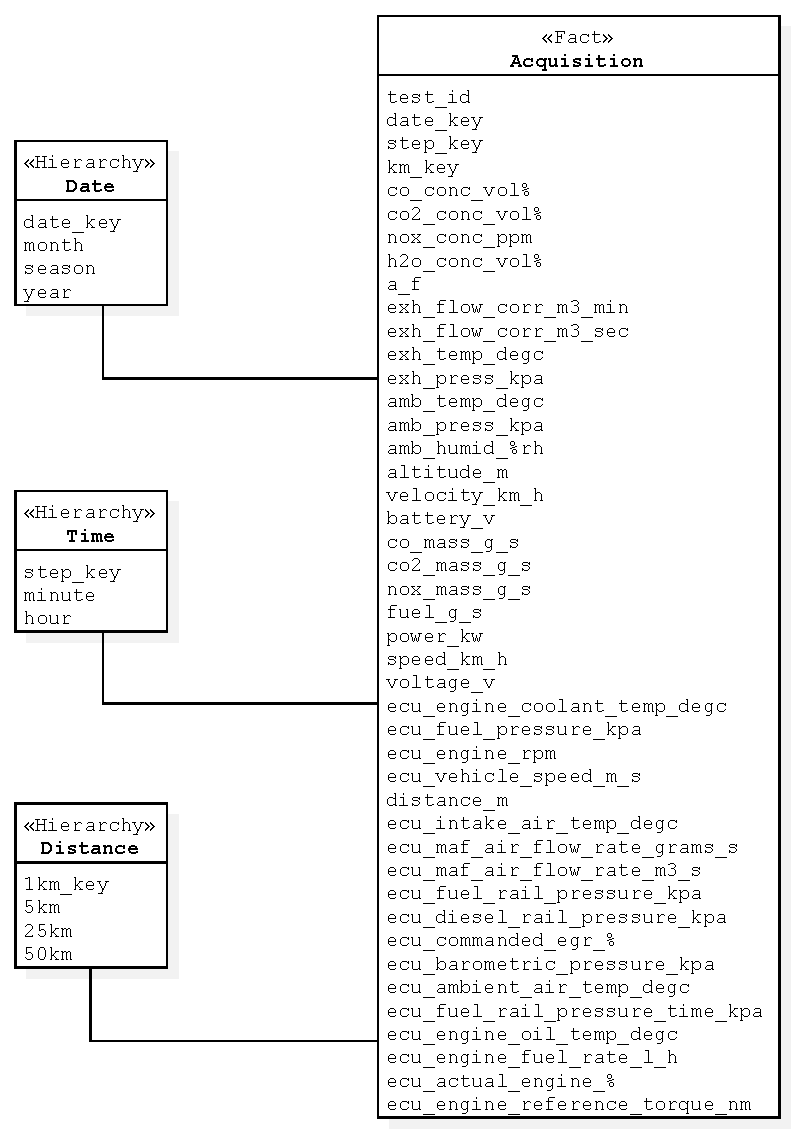
\includegraphics[scale=0.80]{figures/class_fact_scheme}
	\caption{Diagaramma UML schema dei fatti}
	\label{fig:ofm}
\end{figure}
\subsection{Partizionamento Verticale}
È stata inoltre progettata e implementata una variante dello schema proposto che sfrutta la tecnica del partizionamento verticale ovvero la possibilità di dividere la tabella dei fatti in più tabelle, ognuna delle quali rappresenta una particolare sfaccettatura del \textit{fatto}. Il partizionamento viene solitamente adoperato per agevolare quelle interrogazioni che riguardano solo una particolare area di interesse. Per poter applicare questa tecnica è necessario aggiungere una chiave tra le tabelle al fine di poterle ricongiungere per analizzare il dato nella sua completezza.
\begin{figure}[H]
	\centering
	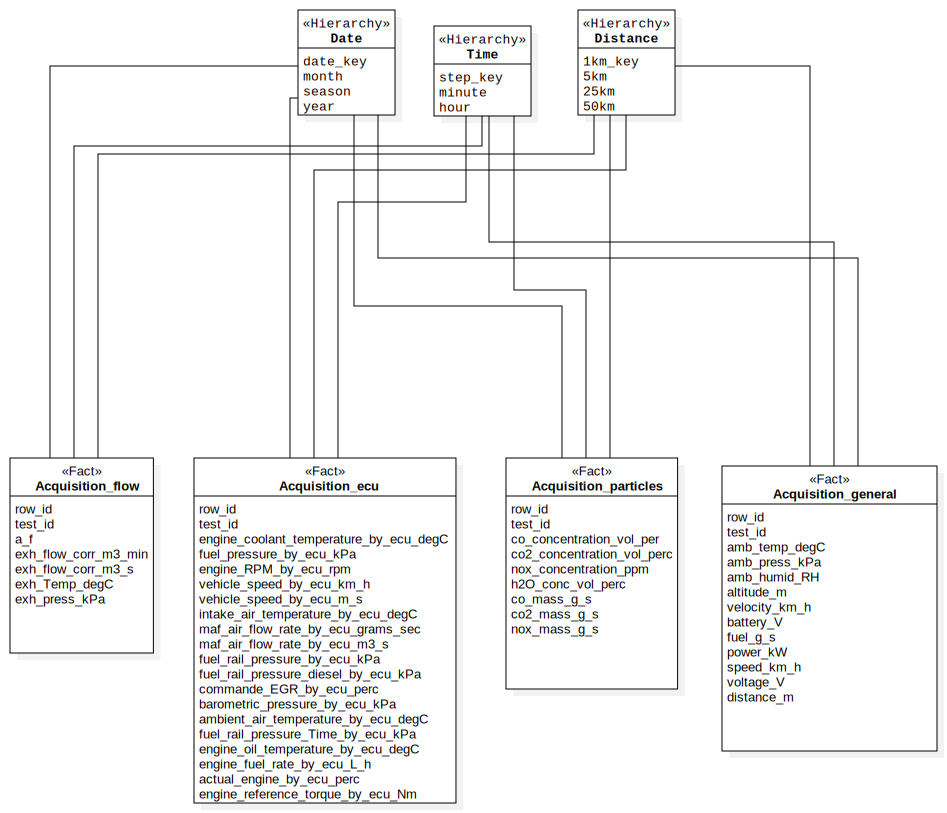
\includegraphics[scale=0.8]{figures/class_fact_scheme_part} %TODO cambiare diagaramma
	\caption{Diagramma UML schema dei fatti partizionato verticalmente}
	\label{fig:ofm}
\end{figure}
\newpage
\section{Extract, Transform, Load}
Al fine di avere un numero rilevante di dati per l'analisi dei tempi è stato implementato un meccanismo di duplicazione dei file.
La procedura ETL sviluppata si compone di differenti passaggi descritti nella seguente tabella.
\begin{table}[H]
	\centering
	\begin{tabular}{clll}
		\rowcolor[HTML]{333333} 
		{\color[HTML]{FFFFFF} \#}	& {\color[HTML]{FFFFFF} Passaggio}	& {\color[HTML]{FFFFFF} Descrizione}	& {\color[HTML]{FFFFFF} Implementazione}
		\\
		1							& \begin{tabular}[c]{@{}l@{}}Trasformazione dei file\\ XLSX in formato CSV\end{tabular}
																		& \begin{tabular}[c]{@{}l@{}}Eliminazione righe inconsistenti\\Calcolo dei campi formula\\Creazione di una data fittizia \\Creazione di un test\_id\\Salvataggio in formato CSV\end{tabular}
																									            & \begin{tabular}[c]{@{}l@{}}Java\end{tabular}
		\\
		\rowcolor[HTML]{C0C0C0} 
		2                         & \begin{tabular}[c]{@{}l@{}}Importazione dei dati in\\ tabella provvisoria\end{tabular} 
																		& \begin{tabular}[c]{@{}l@{}}Viene sfruttata il comando copy\\ del DBMS per importare i dati\\ in maniera efficiente\end{tabular}
																												 & \begin{tabular}[c]{@{}l@{}}PostgreSQL\end{tabular} 
		\\
		3                         & \begin{tabular}[c]{@{}l@{}}Shutdown degli indici\end{tabular}        
																		& \begin{tabular}[c]{@{}l@{}}\end{tabular}
																												 & \begin{tabular}[c]{@{}l@{}}PostgreSQL\end{tabular}
		\\
		\rowcolor[HTML]{C0C0C0} 
		4                         & \begin{tabular}[c]{@{}l@{}}Aggiornamento dello schema\end{tabular}                     
																		& \begin{tabular}[c]{@{}l@{}}Aggiornamento delle dimensioni\\Aggiornamento tabella dei fatti\end{tabular}            
																												 & \begin{tabular}[c]{@{}l@{}}PostgreSQL\end{tabular}	                      
		\\	
		5                         & \begin{tabular}[c]{@{}l@{}}Riattivazione degli indici\end{tabular}             
																		& \begin{tabular}[c]{@{}l@{}}\end{tabular}  
																												 & \begin{tabular}[c]{@{}l@{}}PostgreSQL\end{tabular}    
		\\
		\rowcolor[HTML]{C0C0C0} 
		6                         & \begin{tabular}[c]{@{}l@{}}Aggiornamento viste\end{tabular}                     
																		& \begin{tabular}[c]{@{}l@{}}\end{tabular}            
																												 & \begin{tabular}[c]{@{}l@{}}PostgreSQL\end{tabular}	
	\end{tabular}
\end{table}
\noindent{}Per righe inconsistenti si intendono tutte quelle righe ove per valori indicanti volumi e/o concentrazioni vi sono valori negativi; inoltre viene dedotta la distanza percorsa ove mancante sfruttando la distanza percorsa e le velocità istantanee rilevate negli istanti precedenti.

\section{Viste Materializzate}
Sono state create le seguenti viste materializzate al fine di implementare efficacemente le query \textbf{C} ed \textbf{E}. Il primo frammento dichiara una vista contenente per ogni corsa (\textit{test\_id}) il carburante consumato suddiviso per fasce di velocità.
\lstinputlisting[language=mySQL]{./sources/sql/view_speed.sql}

\noindent{}L'estratto a seguire serve a calcolare una vista materializzata riportante l'efficienza dell'auto nelle diverse corse. I risultati sono stati distribuiti su 3 RPM.
\lstinputlisting[language=mySQL]{./sources/sql/view_rpm.sql}